\begin{activite}[Tout un programme]\label{EQactiTtPrgm}

\begin{partie}[Trois programmes de calculs]\label{EQacti3progs}




Alice et Bertrand saisissent le même nombre de départ sur leurs calculatrices puis effectuent les programmes de calculs suivants : 

\begin{cadre}
Alice multiplie le nombre de départ par 8 puis ajoute 7 au résultat obtenu.
\end{cadre}

\begin{cadre}
Bertrand multiplie le nombre de départ par 6 puis ajoute 13 au résultat obtenu.
\end{cadre}
Ils s'aperçoivent alors que leurs calculatrices affichent le même résultat.
\begin{enumerate}
\item Le nombre 1 est-il leur nombre de départ ? Justifie tes calculs.
\item \label{EQact01} Et le nombre 2 ? Poursuis jusqu'à ce que tu trouves le nombre solution.
Chloé effectue, avec le même nombre de départ qu'Alice et Bertrand, le programme de calculs suivant : 
\begin{cadre}
Chloé multiplie le nombre de départ par 3 puis ajoute 30 au résultat obtenu.
\end{cadre}
\item Trouve-t-elle le même résultat qu'Alice et Bertrand ? Justifie.
\end{enumerate}
\end{partie}


\begin{partie}[Avec un tableur]
Chaque programme de calculs précédent débute maintenant par un même nombre.
\begin{enumerate}
\item Dans un tableur, construis le tableau ci-dessous. Programme la cellule \texttt{B2} en fonction de la cellule \texttt{B1} pour obtenir le résultat de la suite de calculs d'Alice. Copie alors cette formule dans les cellules \texttt{C2} à \texttt{L}2. 
Procède de la même façon pour les programmes de calculs de Bertrand et Chloé. 

\vspace{1em}

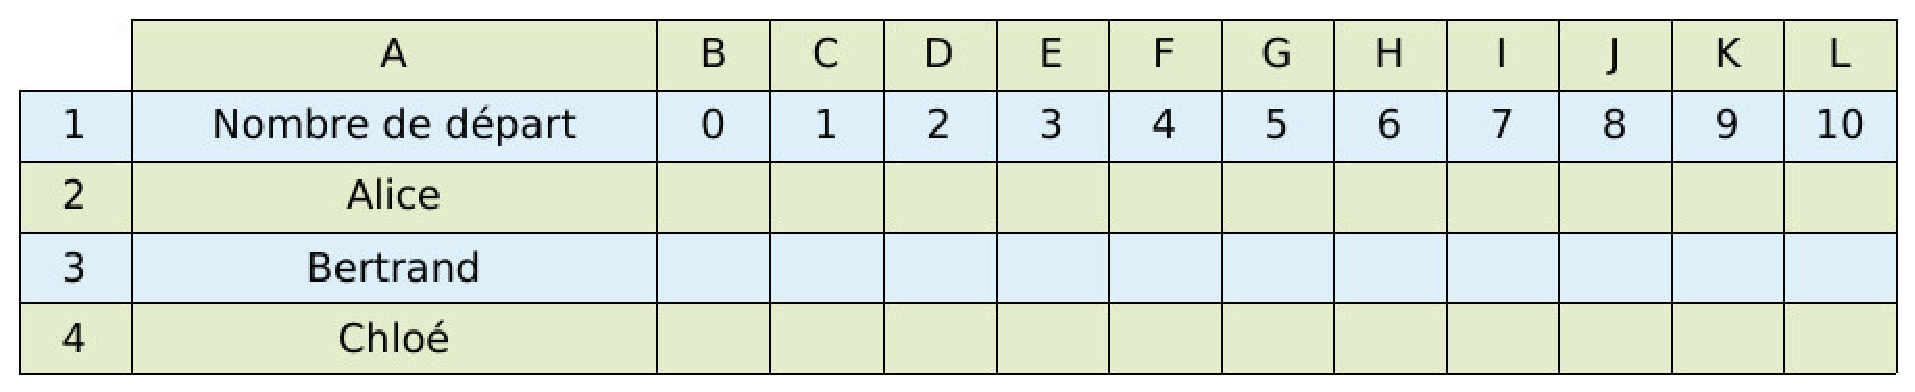
\includegraphics[width=\linewidth]{EqA00}

\vspace{1em}

\item Retrouve la valeur solution de la question \ref{EQact01} de la partie \ref{EQacti3progs}.

\vspace{.5em}

Alice et Chloé cherchent quel nombre afficher sur leurs calculatrices pour trouver le même résultat. 

\vspace{.5em}

\item En t'aidant du tableur, indique les résultats obtenus par Alice et Chloé à la fin de leurs programmes de calculs si elles affichent, sur leurs calculatrices, le nombre 4 au départ. Même question avec le nombre 5. Déduis-en un encadrement du nombre cherché par deux entiers consécutifs.
\item Poursuis en remplaçant les valeurs de la ligne 1 par des valeurs bien choisies puis détermine le nombre solution à afficher sur la calculatrice.

\vspace{.5em}

Bertrand et Chloé cherchent quel nombre afficher sur leurs calculatrices pour trouver le même résultat. 

\vspace{.5em}

\item Procède de la même façon que précédemment pour déterminer un encadrement du nombre solution au millième près. Penses-tu que cette méthode permet de trouver la valeur exacte de ce nombre ?
\item Invente un programme de calculs et cherche, à l'aide du tableur, quel nombre commun afficher sur ta calculatrice et celle de Chloé pour trouver le même résultat. 
\end{enumerate}
\end{partie}
\end{activite}






\begin{activite}[Égalité et opérations]
Ali et Sonia ont le même nombre de billes.
\begin{enumerate}
\item Si tu redonnes autant de billes à Ali et Sonia, en auront-ils toujours le même nombre ?
\item Si tu prends des billes à Ali, que dois-tu faire pour que Sonia en aient le même nombre ?
\item Sonia double son nombre de billes en jouant. Que doit faire Ali pour conserver le même nombre de billes que Sonia ?
\item Ali partage équitablement ses billes en trois paquets. Il en donne deux à ses camarades et en garde un. Sonia décide de faire pareil. Ont-ils toujours le même nombre de billes ?
\item Énonce les propriétés que tu viens de mettre en évidence.
\end{enumerate}
\end{activite}
 
 
 
 
\begin{activite}[Techniques de résolution d'équations]
\begin{enumerate}
\item Recopie puis transforme chaque égalité en une égalité équivalente.

\vspace{1em}

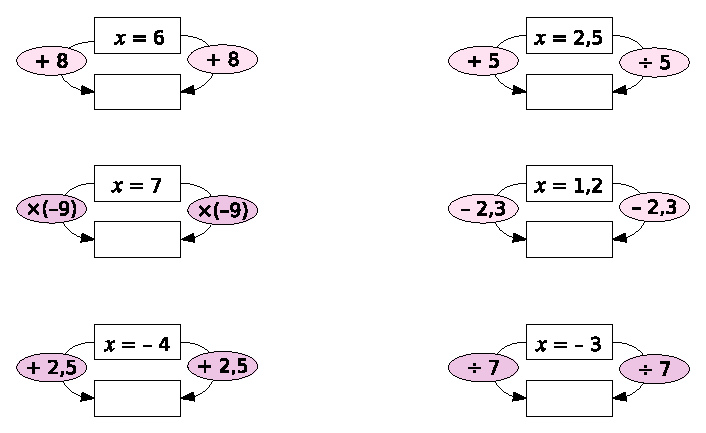
\includegraphics[width=.7\linewidth]{EqA01}

\vspace{1em}


%%%%%%%%
%%%%%%%%  ATTENTION NEWPAGE POUR MISE EN PAGE
%%%%%%%%
\newpage
%%%%%%%%
%%%%%%%%
%%%%%%%%

\item  Le but est de déterminer x dans chacune des équations suivantes. Recopie puis détermine l'opérateur.

\begin{minipage}[c]{.48\linewidth}
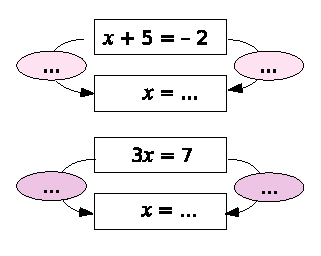
\includegraphics[width=.6\linewidth]{EqA02}
\end{minipage}%
\hfill%
\begin{minipage}[c]{.48\linewidth}
\begin{align*}
\text{On rédige de la façon suivante : } \quad      x + 5 &= -2 \\
                                                x + 5 - 5 &= -2 - 5 \\
                                                        x &= -7 \\
& \\
\text{On rédige de la façon suivante : }  \quad         3x &= 7 \\
                                                    \dfrac{3x}{3}&= \dfrac{7}{3} \\
                                                    x &= \dfrac{7}{3}\\
\end{align*}
\end{minipage}

\item Utilise d'abord les opérateurs pour résoudre les équations suivantes puis rédige comme ci-dessus. Vérifie ensuite que ta solution est juste. 
    \subitem \textbf{a.} $x - 5,2 = 2,6$
    \subitem \textbf{b.} $-6,5x = -14,2$
    \subitem \textbf{c.} $-x = 7,2$
\item De la même façon mais en deux étapes, résous les équations suivantes : 
    \subitem \textbf{a.} $2x + 3 = 5$
    \subitem \textbf{b.} $7x - 6 = -1$
    \subitem \textbf{c.} $2,6 - 5x = -1,4$
\end{enumerate}
\end{activite}
    
    


\begin{activite}[Choix de l'inconnue]
Trois personnes se partagent la somme de 316\,€. On veut trouver la part de chacune sachant que la seconde a 32\,€ de plus que la première et que la troisième a 15\,€ de plus que la seconde. 
\begin{enumerate}
\item Soit $x$ la part de la première personne. Mets ce problème en équation puis résous-le.
\item Soit $x$ la part de la deuxième personne. Mets ce problème en équation puis résous-le.
\item Y a-t-il une autre possibilité pour le choix de l'inconnue ? Si oui, mets ce problème en équation à partir de ce choix puis résous-le.
\item Conclus.
\end{enumerate}
\end{activite}





\begin{activite}[Mise en équation]
On reprend les programmes de calculs des trois camarades de l'Activité \ref{EQactiTtPrgm} :

\begin{cadre}
Alice multiplie un nombre par 8 puis ajoute 7 au résultat obtenu ;
\end{cadre}

\begin{cadre}
Bertrand multiplie un nombre par 6 puis ajoute 13 au résultat obtenu ;
\end{cadre}

\begin{cadre}
Chloé multiplie un nombre par 3 puis ajoute 30 au résultat obtenu.
\end{cadre}

\begin{enumerate}
\item On appelle $x$ le nombre de départ affiché sur les calculatrices d'Alice et Bertrand.
Écris l'équation que doit vérifier $x$ pour que leurs résultats soient les mêmes après avoir effectué chacun leur programme de calculs puis résous-la.
\item On appelle $y$ le nombre de départ affiché sur les calculatrices d'Alice et Chloé.
Écris l'équation que doit vérifier $y$ pour que leurs résultats soient les mêmes après avoir effectué chacun leur programme de calculs puis résous-la.
\item On appelle $z$ le nombre de départ affiché sur les calculatrices de Bertrand et Chloé.
Écris l'équation que doit vérifier $z$ pour que leurs résultats soient les mêmes après avoir effectué chacun leur programme de calculs.
\end{enumerate}
\end{activite}




\begin{activite}[Interprétation du résultat]

\begin{cadre}
Problème 1 : Sylvia a sept ans de plus que sa sœur Rose. Dans 10 ans, Sylvia aura le double de l'âge de Rose. Quel est l'âge de Rose ? Appelle $x$ l'âge de Rose.
\end{cadre}

\begin{cadre}
Problème 2 : En 2000, Paul avait 10 ans et Louis 17 ans. En quelle année, l'âge de Louis a‑t‑il été le double de l'âge de Paul ? Appelle $x$ la différence entre cette année et 2 000.
\end{cadre}

\begin{enumerate}
\item Mets ces deux problèmes en équations. Que remarques-tu ?
\item Résous l'équation. 
\item Déduis-en la solution de chaque problème.
\item Conclus.
\end{enumerate}
\end{activite}
